% file: mybeamer.tex @ https://github.com/zfengg/toolkit/tree/master/tex/mybeamer
%
%	A prefered beamer template for daily presentations.
%
% author: Zhou Feng @ 12/11/2020
% ---------------------------------------------------------------------------- %
%                                   preamble                                   %
% ---------------------------------------------------------------------------- %
\documentclass{beamer}
%[aspectratio=169] % 1610, 149, 54, 43 and 32
%[handout]
%\usepackage{pgfpages}
%\pgfpagesuselayout{2 on 1}[a4paper,border shrink=5mm]
%\pgfpagesuselayout{4 on 1}[a4paper,border shrink=5mm,landscape]

% ----------------------------- themes & packages ---------------------------- %
\usetheme{Warsaw} 
% Warsaw/default/Madrid/default/Darmstadt/Boadilla/Antibes/Hannover/Singapore/Malmoe/Luebeck

%\usecolortheme{crane}	% whale/crane/orchid
\useinnertheme{circles} % circles/rectangles/rounded/inmargin
%\useoutertheme{serif}
%\usefonttheme{shadow} 	% tree


%% headline & footline & nav symbol
%\setbeamercolor{myheadline}{fg=white,bg=blue}
%\setbeamertemplate{headline}{%
%	\leavevmode%
%	\begin{beamercolorbox}[wd=\paperwidth,ht=3ex,dp=1.125ex]{frametitle}%
%	\centering \footnotesize\color{white}\insertsection\par
%	\end{beamercolorbox}%
%}
\setbeamertemplate{headline}{}

\beamertemplatenavigationsymbolsempty 						% remove the navigation bar
%\setbeamertemplate{navigation symbols}{}				% headline, symbols
\setbeamertemplate{footline}[frame number]			% remove footline
%\setbeamertemplate{footline}{
%	\usebeamercolor[fg]{page number in head/foot}%
%	\usebeamerfont{page number in head/foot}%
%	\quad {\hhmm \tdtime} \hfill
%	\setbeamertemplate{page number in head/foot}[framenumber]%
%	\setbeamertemplate{page number in head/foot}[totalframenumber]
%	\usebeamertemplate*{page number in head/foot}\kern1em\vskip2pt%
%}


%\setbeamertemplate{section in toc}[sections numbered]		% style of section in toc
%\setbeamertemplate{subsection in toc}[triangle unnumbered] % style of subsection in toc, ball/square/circle/default
%\setbeamertemplate{sections/subsections in toc}[circle]	% style of sec/subsec in toc
%\setbeamertemplate{items}[default] 						% chevron/default


%\usepackage{tikz}											% draw advanced graphics in latex
%\pgfdeclareimage[height=0.5cm]{university−logo}{.data/MapQM.pdf}
%\logo{\pgfuseimage{university−logo}}

%\usepackage[orientation=landscape,size=custom,width=16,height=9,scale=0.5,debug]{beamerposter} % change the size of beamer

%\usepackage[font=Times,
%			timeinterval=59,
%			timeduration=3,
%			timewarningfirst=90]{tdclock}

% -------------------------- hyperlinks & bookmarks -------------------------- %
\hypersetup{pdfusetitle,
			colorlinks=false,
			linkcolor=blue,
			citecolor=blue,
			urlcolor=black}

% -------------------------------- environment ------------------------------- %
\newtheorem{conjecture}{Conjecture}

% --------------------------------- citations -------------------------------- %
\usepackage{natbib}

% ----------------------------------- misc ----------------------------------- %
\allowdisplaybreaks

% -------------------------------- fast-typing ------------------------------- %

% special for this article

% --------------------------------- titlepage -------------------------------- %
\title[Short Title]{My Beamer Template}
\subtitle{A subtitle}
\author[Z. Feng]{Zhou Feng}
\institute[CUHK]{The Chinese University of Hong Kong}
\date{\today}
%	\\ \vspace{1em}
%	\footnotesize{Joint work with A and B}}


% ---------------------------------------------------------------------------- %
%                                   document                                   %
% ---------------------------------------------------------------------------- %

\begin{document}
	
\begin{frame}[plain]
%	\initclock
	\maketitle
\end{frame}

\begin{frame}\label{contents}
	\frametitle{Outline}
	\tableofcontents
\end{frame}


\section{Introduction} \label{sec:intro}

\subsection{Basic Environments}
\begin{frame}
	\frametitle{List}
	\begin{itemize}
		\item Point A
		\item Point B
		      \begin{itemize}
			      \item Subpoint C
		      \end{itemize}
	\end{itemize}

	\begin{enumerate}
		\item Point 1 \pause
		\item Point 2
		      \begin{enumerate}[I]
			      \item Analysis
			      \item Algebra
			      \item Geometry
			      \item Combinatorics
		      \end{enumerate}
		\item
		      \begin{enumerate}[i]
			      \item $ \alpha $
			      \item $ \beta $
		      \end{enumerate}
	\end{enumerate}

\end{frame}

\begin{frame}{Citations}
	
	\begin{itemize}
		\item \structure{\citep{Bowen1975}}
		
		\item \structure{\cite{BreuillardVarju2020}}
		
		\item \citep*{AkiyamaEtAl2020}
		
		\item \citet*{AkiyamaEtAl2020}
		
		\item \citealp*{BaranyEtAl2019}
		
		\item \citeauthor{BarralFeng2021}
		
		\item \citeauthor{BarreiraEtAl1999}
		
		\item \citeauthor{Erdoes1939}
	\end{itemize}
	
\end{frame}


\begin{frame}
	\frametitle{Description}
	\begin{description}
		\item[API] Application programming interface
		\item[LAN] Local Area Network
		\item[ASCII] American Standard Code for Information Interchange
	\end{description}
\end{frame}

\begin{frame}
	\frametitle{Tables}
	\begin{table}
		\centering
		\begin{tabular}{l | c | c | c | c }
			Competitor Name & Swim  & Cycle & Run   & Total \\
			\hline 
			John T          & 13:04 & 24:15 & 18:34 & 55:53 \\
			Norman P        & 8:00  & 22:45 & 23:02 & 53:47 \\
			Alex K          & 14:00 & 28:00 & n/a   & n/a   \\
			Sarah H         & 9:22  & 21:10 & 24:03 & 54:35
		\end{tabular}
		\caption{Triathlon results}
		\label{tab:1}
	\end{table}
	
\end{frame}

\begin{frame}
	\frametitle{Blocks}
	\begin{block}<1->{Block Title}
		Lorem ipsum dolor sit amet, consectetur adipisicing elit,
		sed do eiusmod tempor incididunt ut labore et
		dolore magna aliqua.
	\end{block}
	\begin{alertblock}<3->{Block Title}
		Lorem ipsum dolor sit amet, consectetur adipisicing elit,
		sed do eiusmod tempor incididunt ut labore et
		dolore magna aliqua.
	\end{alertblock}
	\begin{definition}
		A prime number is a number that...
	\end{definition}
	\begin{example}<2->[\citealp{Bowen1975}]
		Lorem ipsum dolor sit amet, consectetur adipisicing elit,
		sed do eiusmod tempor incididunt ut labore et
		dolore magna aliqua.
	\end{example}
\end{frame}


\begin{frame}{Theorems and Corollaries}

	\begin{theorem}[Pythagoras]
		$ a^2 + b^2 = c^2$
	\end{theorem}

	\begin{theorem}[\citealp*{AkiyamaEtAl2020}]
		content
	\end{theorem}

	\begin{corollary}
		$ x + y = y + x  $
	\end{corollary}
	\begin{proof}
		$\omega +\phi = \epsilon $
	\end{proof}
\end{frame}


\begin{frame}
	\frametitle{Columns}
	\begin{columns}
		\column{0.5\textwidth}
		Classical Mechanics
		
		Electromagnetism
		
		Special Relativity
		
		General Relativity
		
		Quantum Mechanics
		
		Quantum field theory
		
		Particle Physics, Standard model
		
		Statistic Physics, Thermodynamics.

		\column{0.5\textwidth}
%		\begin{figure}
%			\centering
%			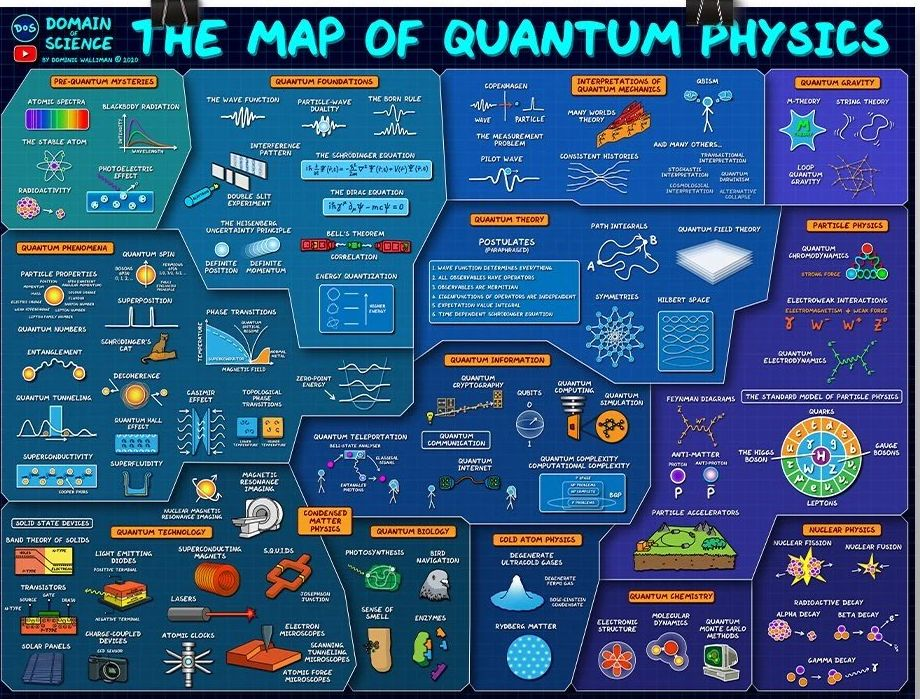
\includegraphics[width=\columnwidth]{./data/MapQM.jpg}
%		\end{figure}

	\end{columns}

\end{frame}


\begin{frame}
	\frametitle{Buttons}
	\hyperlink{contents}{\beamerbutton{contents page}}
	\hyperlink{contents}{\beamergotobutton{columns page}}
	\hyperlink{contents}{\beamerskipbutton{pictures page}}
	\hyperlink{contents}{\beamerreturnbutton{pictures page}}
\end{frame}



\section{Animation}


\begin{frame}
	\frametitle{Overlays}
	\onslide<1->{First Line of Text}

	\onslide<2->{Second Line of Text}

	\onslide<3->{Third Line of Text}
\end{frame}

\setbeamercovered{transparent}
\begin{frame}
	\frametitle{Overlays}
	\uncover<1->{First Line of Text}

	\uncover<2->{Second Line of Text}

	\uncover<3->{Third Line of Text}
\end{frame}

\begin{frame}
	\frametitle{Overlays}
	\only<1>{First Line of Text}

	\only<2>{Second Line of Text}

	\only<3>{Third Line of Text}
\end{frame}


\begin{frame}
	\frametitle{Text formatting}
	\textbf<2>{Example Text}

	\textit<2>{Example Text}

	\textsl<2>{Example Text}

	\textrm<2>{Example Text}

	\textsf<2>{Example Text}

	\textcolor<2>{orange}{Example Text}

	\alert<2>{Example Text}

	\structure<2>{Example Text}
\end{frame}

\begin{frame}{Print some meta-info}
	\begin{itemize}
		\item \insertframenumber
		\item \insertauthor
		\item \insertinstitute
		\item \insertshortauthor
		\item \insertshortinstitute
		\item \inserttitle
		\item \insertshorttitle
	\end{itemize}
\end{frame}

\begin{frame}
\begin{center}
	\large
	Thank you for listening!
\end{center}
\end{frame}


% ---------------------------------------------------------------------------- %
%                                   reference                                  %
% ---------------------------------------------------------------------------- %

\begin{frame}<presentation:0>[allowframebreaks,noframenumbering]{Reference}
	\bibliographystyle{myabbrvnat}
	\bibliography{mybeamer}
\end{frame}

\end{document}
